\documentclass[        
    a4paper,          % Tamanho da folha A4
    12pt,             % Tamanho da fonte 12pt
    chapter=TITLE,    % Todos os capitulos devem ter caixa alta
    section=Title,    % Todas as secoes devem ter caixa alta somente na primeira letra
    subsection=Title, % Todas as subsecoes devem ter caixa alta somente na primeira letra
    oneside,          % Usada para impressao em apenas uma face do papel
    english,          % Hifenizacoes em ingles
    spanish,          % Hifenizacoes em espanhol
    brazil,           % Ultimo idioma eh o idioma padrao do documento
    sumario=abnt-6027-2012,
]{abntex2}



\usepackage{graphicx}                               % Inserir figuras
\usepackage[utf8]{inputenc}                         % Acentuação direta
\usepackage[T1]{fontenc}
\usepackage{lmodern}

\usepackage{amsfonts, amssymb, amsmath}             % Fonte e símbolos matemáticos
\usepackage{booktabs}                               % Comandos para tabelas
\usepackage{verbatim}                               % Texto é interpretado como escrito no documento
\usepackage{multirow, array}                        % Múltiplas linhas e colunas em tabelas
\usepackage{indentfirst}                            % Endenta o primeiro parágrafo de cada seção.
\usepackage{listings}                               % Utilizar codigo fonte no documento
\usepackage{xcolor}
\usepackage{microtype}                              % Para melhorias de justificação?
\usepackage[portuguese,ruled,lined]{algorithm2e}    % Escrever algoritmos
\usepackage{float}
\usepackage{algorithmic}                            % Criar Algoritmos  
%\usepackage{float}                                 % Utilizado para criação de floats
\usepackage{amsgen}
\usepackage{lipsum}                                 % Usar a simulação de texto Lorem Ipsum
%\usepackage{titlesec}                              % Permite alterar os títulos do documento
\usepackage{tocloft}                                % Permite alterar a formatação do Sumário
\usepackage{etoolbox}                               % Usado para alterar a fonte da Section no Sumário
\usepackage[acronym,nogroupskip,nonumberlist]{glossaries}   % Permite fazer o glossario
\usepackage[alf, abnt-emphasize=bf, recuo=0cm, abnt-etal-cite=2, abnt-etal-list=0, abnt-etal-text=it]{abntex2cite}  % Citações padrão ABNT
\usepackage{makecell}

\renewcommand{\thesection}{\arabic{section}}


\newcommand{\EMPRESA}{Prefeitura de InovCity}
\newcommand{\CIDADE}{InovCity}
\newcommand{\PDTI}{PDTI – Plano Diretor de Tecnologia da Informação}
     
\sloppy

\title{PLANO DIRETOR DE TECNOLOGIA DA INFORMAÇÃO - \MakeUppercase{\EMPRESA{}} - 2017/2019}

\begin{document} 

\maketitle

\vfill
\begin{figure}[!ht]
    \centering
    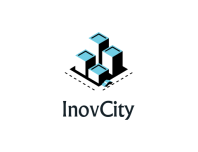
\includegraphics[width=4cm]{figuras/logo.png}
\end{figure}
\vfill    
\vfill

\newpage

\begin{table}[h]
\centering{Histórico de Alterações}
\resizebox{\textwidth}{!}{  
	\begin{tabular}{|l|l|l|l|}
	\hline
	Data & Versão & Descrição & Autor \\ \hline
	14/10/2016 & 0.1 & Defini\c{c}\~ao inicial do documento & Marciano Machado Saraiva e Elisa do Nascimento Hino  \\ \hline
	\end{tabular}
}
\end{table}

\begin{KeepFromToc}
  \tableofcontents
\end{KeepFromToc}

\section{Apresenta\c{c}\~ao}

\subsection{Objetivo}
O objetivo do presente Plano Diretor é, justamente, identificar formas e mecanismos de atender aos Princípios da Estratégia da 
institui\c{c}\~ao, por meio da Tecnologia da Informação e Comunicações, atuando de forma interna (focada nas necessidades e objetivos da 
administração pública municipal) e de forma externa (focada nas necessidades diretas de cidadãos e organizações sediadas em \CIDADE). Tais 
princípios consolidaram-se da seguinte forma:

\begin{itemize}
	\item SUSTENTÁVEL - Desenvolva com equilíbrio ambiental, social e econômico.
	\item HUMANA - Amplie conquistas sociais, cidadania, acessibilidade e qualidade de vida com valorização de suas identidades e cultura.
	\item INTEGRADA - Supere efeitos da divisão territorial da cidade e desenvolva suas potencialidades de forma conjunta.
	\item INOVADORA - Se insira nos setores e tendências de maior dinâmica global, além de consolidar a vocação de cidade inovadora e 
intensa em conhecimento.
	\item PRÓSPERA Desenvolva suas atividades econômicas, gerando mais e melhores oportunidades de trabalho de qualidade e renda para os 
canoenses.
	\item ATRATIVA - \CIDADE{} como referência em cidade metropolitana na atração de investimentos, visitantes e atenção à cidade na oferta 
de qualidade de vida e desenvolvimento sustentável a seus cidadãos
\end{itemize}


\subsection{Abrang\^encia}
A abrangência deste \PDTI{} alcança todas os setores da \EMPRESA{} por constituir o Plano Tático para a execução das ações de TIC na 
Instituição, englobando toda e qualquer política, diretrizes, estratégia, iniciativas que digam respeito à Tecnologia da Informação e 
Comunicação da \EMPRESA{} .
\subsection{Per\'iodo de Validade}
Este \PDTI tem suas metas e objetivos traçados para o período compreendido entre janeiro de 2017 a dezembro de 2019, devendo passar 
por algumas revisões técnicas ao longo deste período.
\subsection{Per\'iodo de Revis\~ao}
O \PDTI poderá ser revisto a cada seis meses, a partir de janeiro de 2017, de forma a sempre refletir as reais necessidades da Instituição, 
seu alinhamento com o negócio, e sua adequação ao processo orçamentário da \EMPRESA{}.

\section{Introdução}
As melhores práticas relacionadas à governança de TI recomendam que qualquer
instituição, pública ou privada, para que possa realizar uma gestão eficiente dos recursos da área
de TI, necessita contar com um planejamento no qual estejam relacionadas todas as metas da
instituição associadas às ações que a área de TI terá que executar para o alcance daquelas metas.
Assim, um Plano Diretor de Tecnologia da Informação (PDTI) representa um instrumento
indispensável para a gestão dos recursos de TI. Os órgãos de controle de governo, em especial o
Tribunal de Contas do Estado (TCE), há muito vêm enfatizando a necessidade dos órgãos públicos
elaborarem um PDTI que contemple todas as ações e as associem às metas de suas áreas de
negócio antes de executarem seus gastos relacionados à TI.
Sendo a Tecnologia da Informação tão importante para as organizações, torna-se
necessário entender as atividades empresariais e os objetivos estratégicos, eventualmente já
traçados pela instituição. Neste sentido, o planejamento estratégico é o responsável pela tomada
de decisão relativa aos objetivos, metas, recursos, planejamento e controle da organização.
Geralmente a quantidade de julgamento no processo decisório é muito alta e é representada pela
alta administração.
Em muitas instituições as decisões de TI são tomadas de forma isolada, por diferentes
motivos e pessoas dentro de sua estrutura. Assim, normalmente, o planejamento estratégico e
tático integrado do ambiente de TI é colocado em segundo plano, ou nem mesmo é realizado.
A elaboração de um PDTI, neste contexto, traz um rico conjunto de questionamentos,
reflexões e revisões que resultará no amadurecimento da TI e da própria instituição. Dentre as
evoluções esperadas, pode-se citar:
\begin{itemize}
 \item Reflexões sobre a missão e visão de futuro da unidade de TI, alinhadas à missão e visão de futuro da instituição;
 \item Busca de respostas às oportunidades e ameaças externas e aos pontos fracos e fortes internos, de modo a cumprir suas atribuições com 
 \item Identificação, revisão e explicitação dos objetivos, orientações estratégicas e recomendações para a TI, alinhados aos 
objetivos estratégicas na organização, e decorrentes planos de ação atrelados às necessidades das áreas de negócio; efetividade;
 \item Identificação e explicitação não apenas das ações operacionais a serem realizadas pela área de TI, mas também dos aspectos de 
estrutura e gestão sobre a TI, em especial pela operacionalização de uma estrutura de governança que viabilizará a execução das ações e
a revisão periódica do PDTI aprovado;
 \item Desenvolvimento de capacidades que fortaleçam e assegurem a execução dos planos eprojetos de TI. 
\end{itemize}


\section{Estrutura Organizacional}
A TIC da \EMPRESA{} encontra-se organizada Coordena\c{c}\~ao de Suporte Técnico com o Assistente de TIC. Veja na 
\autoref{organograma_geral} o organograma geral da institui\c{c}\~ao.

\begin{figure}[H]
    \centering
    \caption{Organograma Geral da Institui\c{c}\~ao}\label{organograma_geral}
    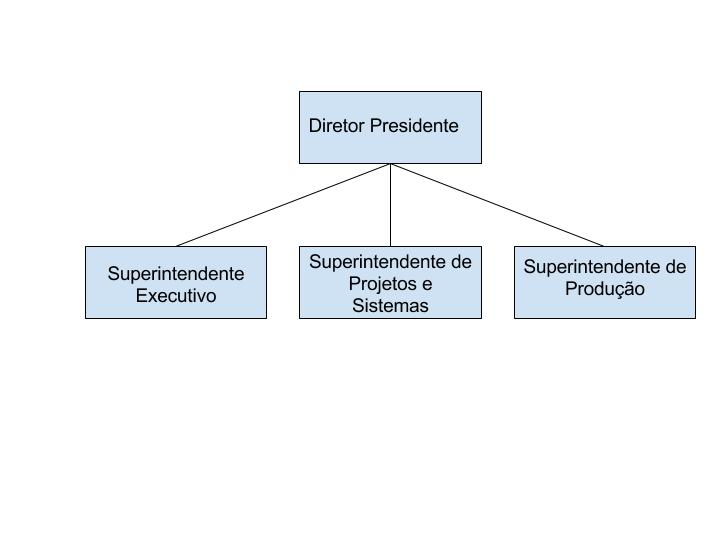
\includegraphics[width=10cm]{figuras/organograma_antes}
\end{figure}


O \textbf{Diretor Presidente} terá a responsabilidade de representar a \EMPRESA{}, judicial e extrajudicialmente, bem como responder por 
todos os atos de gestão.

Ao \textbf{Superintendente Executivo} compete representar o Diretor Presidente em sua falta e executar outras atividades definidas pelo 
Diretor Presidente.

Ao \textbf{Superintendente de Projetos e Sistemas} compete gerir o desenvolvimento dos sistemas de informações utilizados pela Prefeitura 
sejam os mesmos desenvolvidos no ambiente interno ou contratados junto a terceiros, gerir as políticas de segurança, gerir os aplicativos 
utilizados pelo Município, emitir parecer sobre a viabilidade e oportunidade de novas contratações de serviços de tecnologia da informação 
e comunicação, gerar laudos de entregas e certificação de todas as contratações feitas pelo Poder Executivo Municipal, relativas à área de 
TIC, gestão de indicadores de sistemas, de projetos e de segurança, gerar e manter a documentação atualizada dos sistemas,
preparar plano anual de atividades e plano diretor de informática para projetos, sistemas e segurança e executar outras atividades 
definidas pelo Diretor Presidente.

Ao \textbf{Superintendente de Produção} compete manter a infraestrutura de tecnologia de comunicação e os sistemas corporativos 
disponíveis, gerar e gerir o orçamento de Infraestrutura e comunicação, manter o atendimento aos usuários, gerar indicadores de 
disponibilidade de cada
um dos itens de sua responsabilidade, gerar e manter a documentação atualizada do ambiente computacional, apoiar na definição, documentar e 
gerar laudos de entregas e certificação de todas as contratações efetuadas no âmbito do Poder Executivo Municipal, relativas à área de TIC,
preparar plano anual de atividades e plano diretor de informática para área de infraestrutura e executar outras atividades definidas pelo 
Diretor Presidente.

\section{Referencial Estratégico de TI}
\subsection{Miss\~ao}
Gerenciar e assessorar o Poder Executivo Municipal em todos os aspectos relacionados à tecnologia da informação e comunicação, com foco no 
interesse coletivo e utilidade pública, provendo soluções inovadoras e sustentáveis.
\subsection{Vis\~ao}
Ser referência em Gestão de Tecnologia da Informação e Comunicação para a Administração Pública, a nível nacional.
\subsection{Valores}
Transparência, ética, respeito, sustentabilidade, inovação e comprometimento.
\subsection{Análise de SWOT}

A Análise SWOT é uma ferramenta utilizada para fazer análise de cenário interno e externo (ou análise de ambiente), sendo usado como base 
para gestão e planejamento estratégico de uma organização. Trata-se de um método que possibilita verificar e avaliar os
fatores intervenientes para um posicionamento estratégico da Unidade de TI no ambiente em questão.

Tem como objetivos principais efetuar uma síntese das análises internas e externas, identificar elementos chave para a gestão, o que 
implica estabelecer prioridades de atuação e preparar opções estratégicas: análise de riscos e identificação de problemas a serem 
resolvidos.

Ao longo da elaboração deste PDTI, foi realizado um trabalho no sentido de identificar as forças e as fraquezas dos processos internos de 
competência da \EMPRESA{}, seguido da identificação das oportunidades decorrentes de fatores favoráveis verificados no ambiente da
Prefeitura Municipal de \CIDADE{}, bem como as ameaças decorrentes de fatores desfavoráveis e mudanças sazonais ou permanentes do ambiente 
externo.

O resultado dos estudos realizados permite entender melhor o ambiente organizacional da Tecnologia de Informação e auxilia na busca de 
formas de se evoluir a gestão, corrigindo as fraquezas e ameaças encontradas e alavancando as forças e oportunidades identificadas.

A tabela a seguir apresenta o resultado da análise dessas atividades.

\begin{table}[H]
\centering
\caption{Ambientes} \label{my-label}
\resizebox{\textwidth}{!}{ 
\begin{tabular}{|l|l|}
\hline
\multicolumn{1}{|c|}{\textbf{AMBIENTE INTERNO/Forças}} & \multicolumn{1}{c|}{\textbf{AMBIENTE EXTERNO/Oportunidades}} \\ \hline
\begin{tabular}[c]{@{}l@{}}- Equipe altamente comprometida e capacitada tecnicamente\\ - Competências da área de TI mapeadas\\ - Gestores 
qualificados\\ - Conhecimento dos processos operacionais da Prefeitura de InovCity\\ - Estrutura de servidores (hardware) atualizada\\ - 
Unidades de armazenamento (storages) atualizadas\\ - Aplicação de virtualização de servidores\end{tabular} & \begin{tabular}[c]{@{}l@{}}- 
Utilização de novas tecnologias, tais como computação em nuvem e mobilidade\\ - Disponibilidade de recursos de Programas Federais com vistas 
à \\ qualificação dos serviços públicos\end{tabular} \\ \hline
\end{tabular}
}
\end{table}

\begin{table}[H]
\centering
\caption{Fraquezas e Amea\c{c}as}\label{my-label}
\resizebox{\textwidth}{!}{ 
\begin{tabular}{|l|l|}
\hline
\multicolumn{1}{|c|}{\textbf{Fraquezas}} & \multicolumn{1}{c|}{\textbf{Ameaças}} \\ \hline
\begin{tabular}[c]{@{}l@{}}- Sistemas de informações não completamente integrados\\ - Redundância de dados embora pouca, existe\\ - 
Documentação praticamente inexistente\\ - Processos e controles de governança de TI não definidos\\ - Inexistência de planejamento e 
controle orçamentário de TI\\ - Equipamentos de rede obsoletos\end{tabular} & \begin{tabular}[c]{@{}l@{}}- Restrições orçamentárias\\ - 
Dificuldade de adaptação e mudança de cultura pelas áreasde negócios aos novos \\ direcionamentos de gestão de TI. \\ - Demandas não 
planejadas \\ - Áreas de TI independentes nas secretarias Altadependência do fornecedor do sistema de gestão\end{tabular} \\ \hline
\end{tabular}
}
\end{table}


\section{Alinhamento com a Estratégia da Organização}
Esta seção demonstra o alinhamento das estratégias de TIC da \EMPRESA{}, presentes no \PDTI{}, com as principais políticas e planos
governamentais.

\begin{figure}[H]
    \centering
    \caption{Antigo Mapa Estratégico da \EMPRESA{}}\label{mapa_estrategico_2016}
    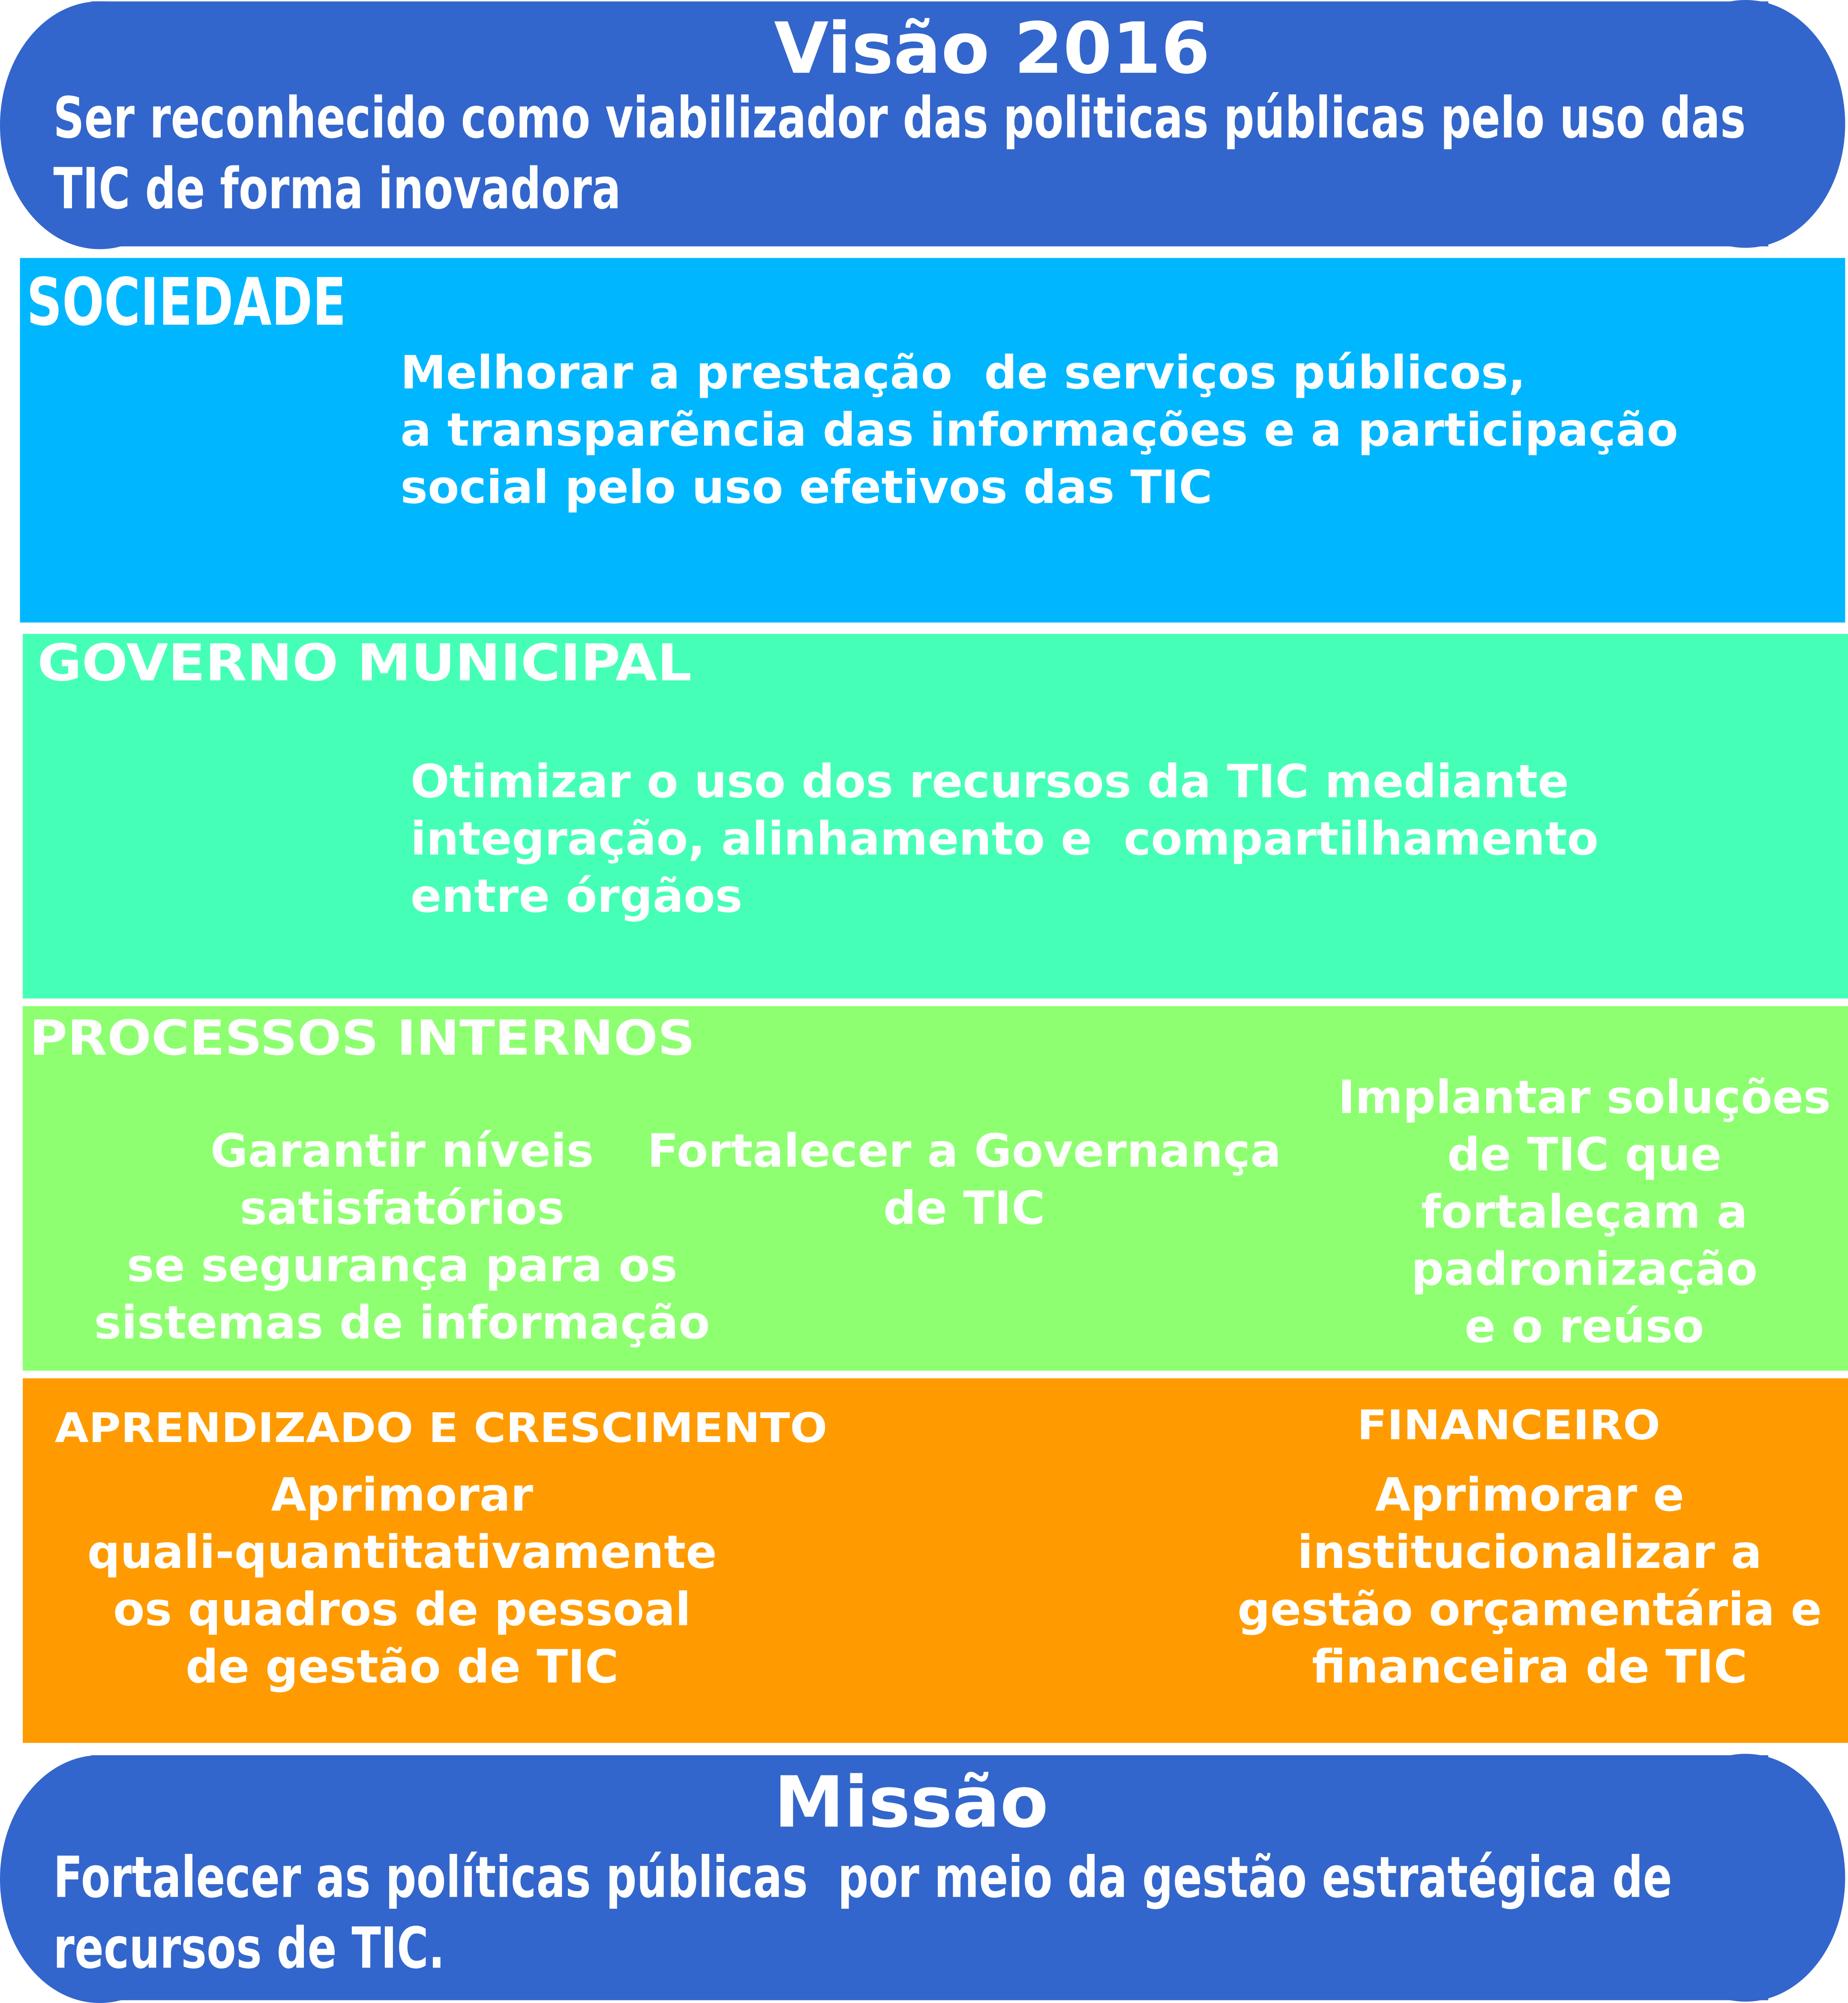
\includegraphics[width=10cm]{figuras/mapa_estrategico_2016.png}
\end{figure}

\begin{figure}[H]
    \centering
    \caption{Novo Mapa Estratégico para a \EMPRESA{}}\label{mapa_estrategico_2017_19}
    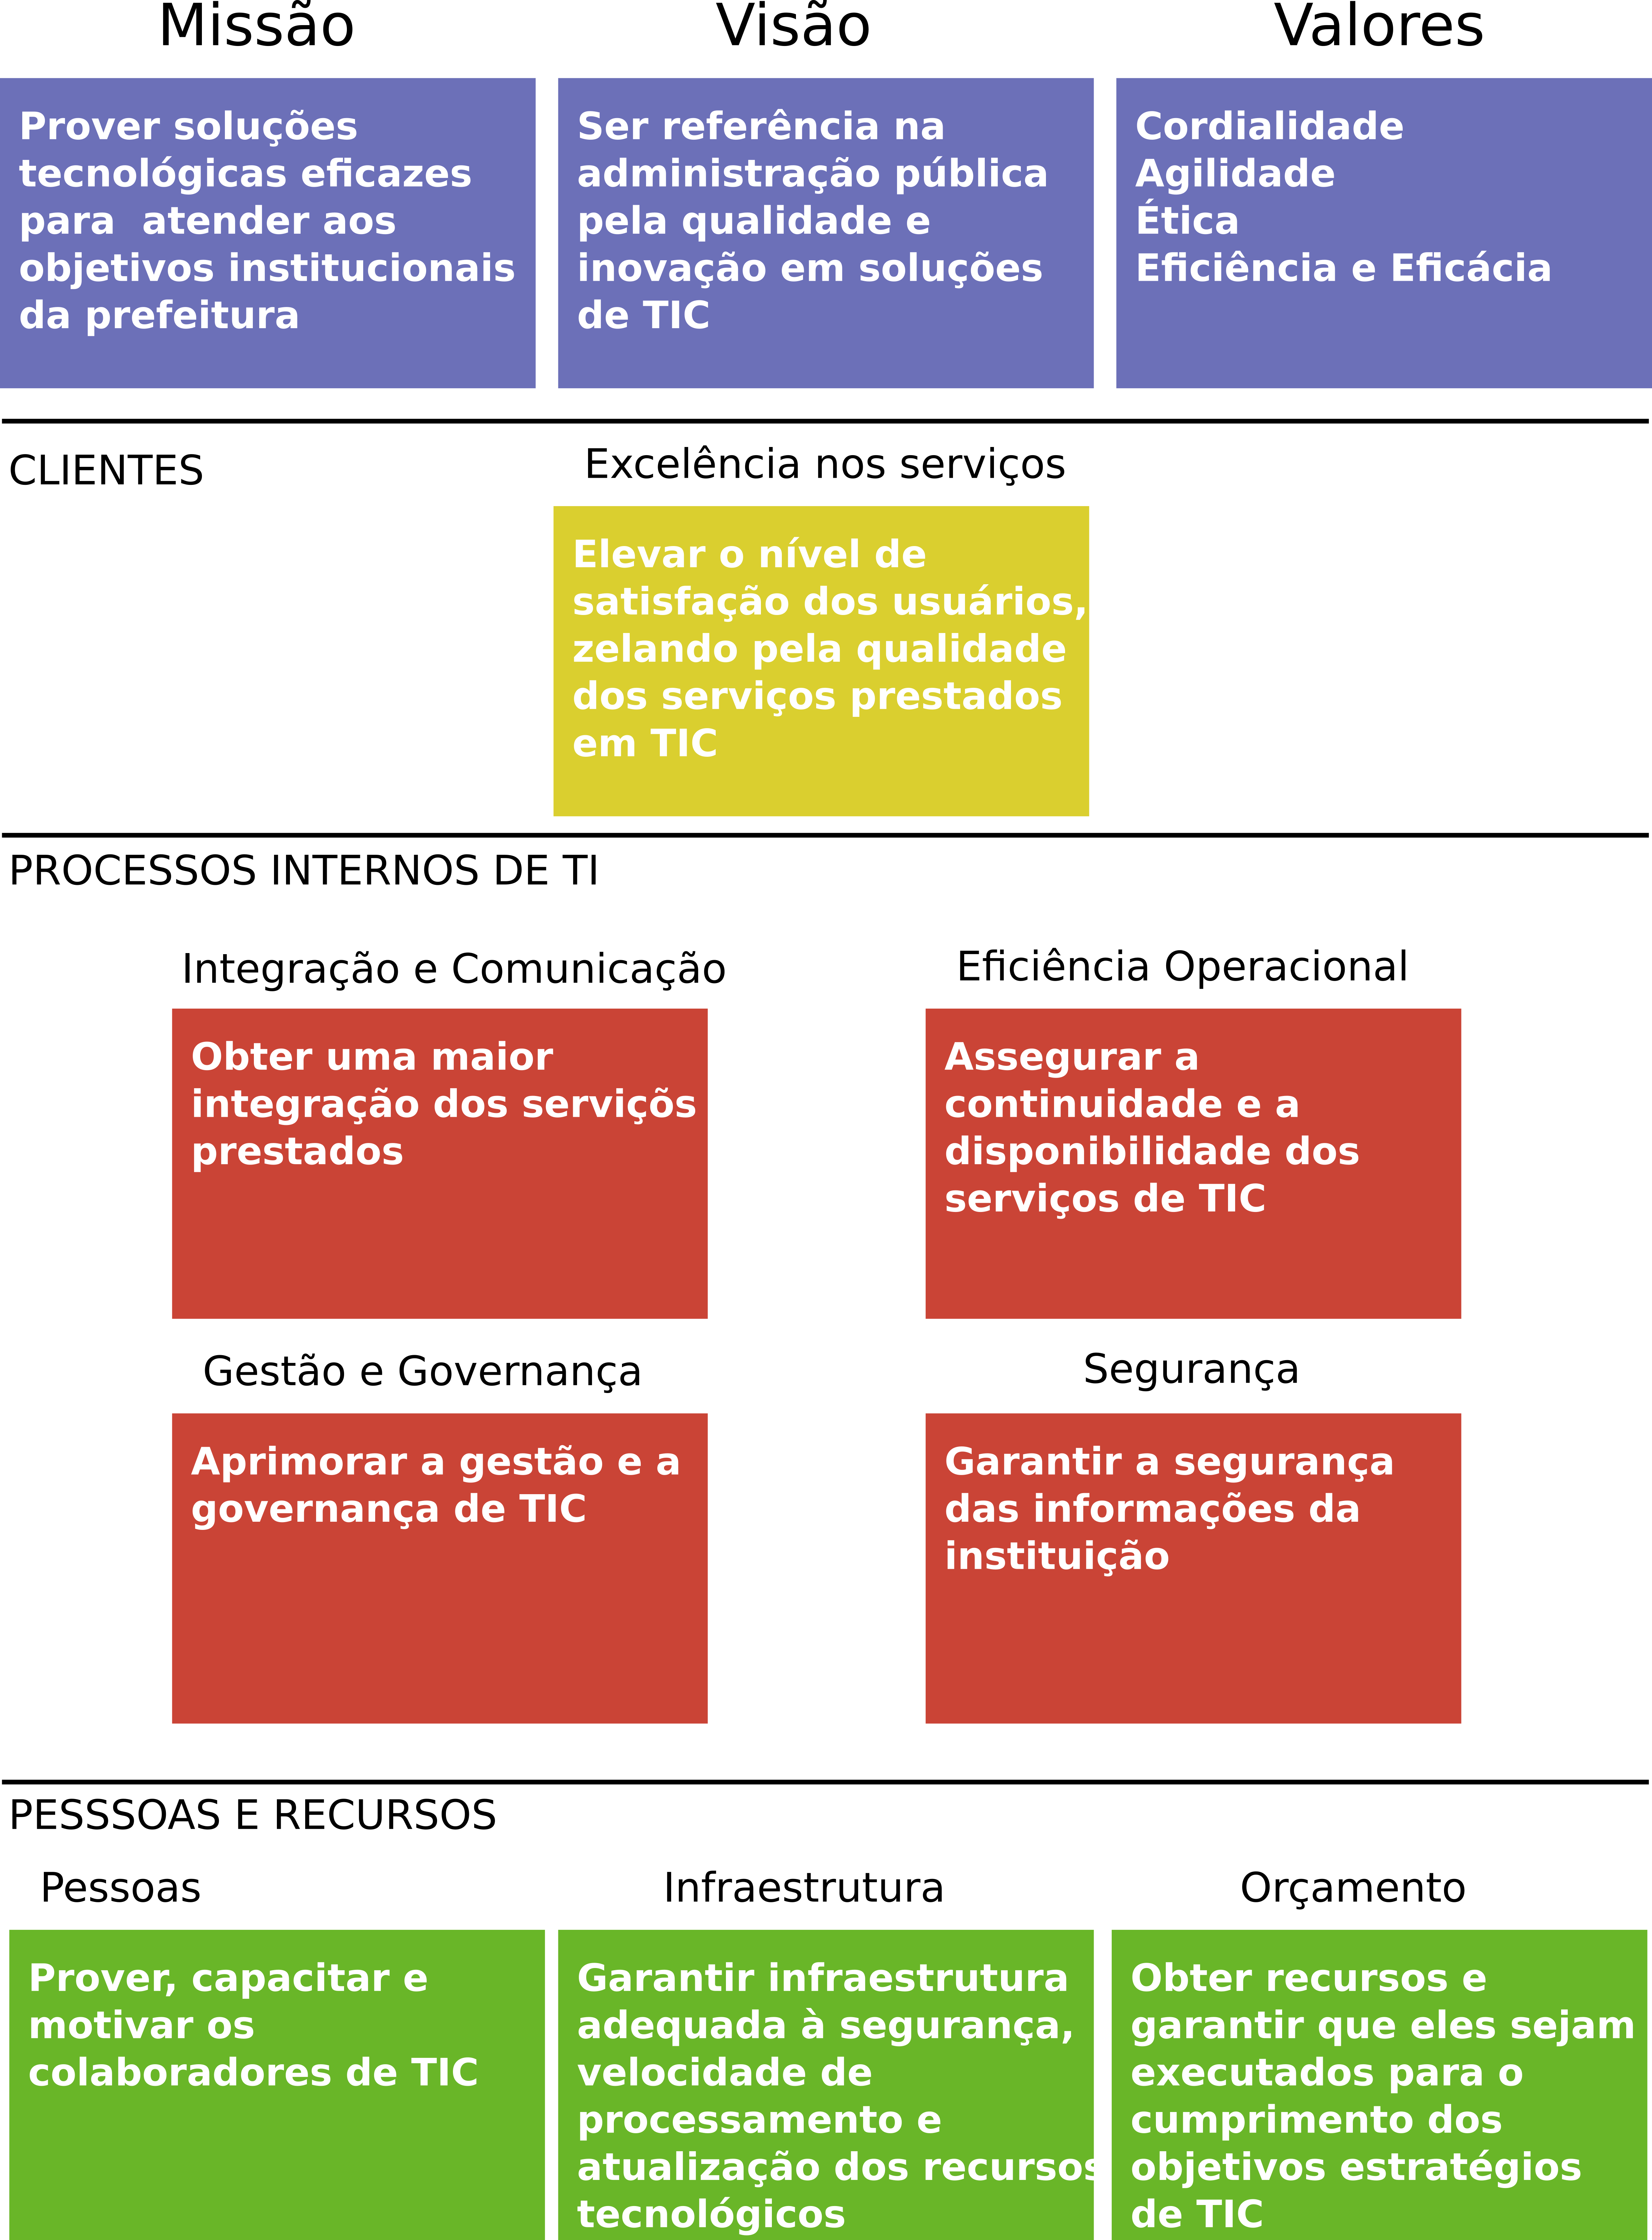
\includegraphics[width=10cm]{figuras/mapa_estrategico_2017_19.png}
\end{figure}

\section{Inventário de Necessidades}
As necessidades de TI foram agrupadas pelas seguintes categorias: sistemas de
informações (SI); serviços de TI (SE); infraestrutura (IN); infraestrutura de sistemas (IS);
contratação de serviços de terceiros (T); e organização e pessoal (PO). 

\begin{table}[H]
\centering
\caption{Necessidades de TI}
\label{my-label}
\begin{tabular}{|l|l|}
\hline
\multicolumn{1}{|c|}{\textbf{ID}} & \multicolumn{1}{c|}{\textbf{NECESSIDADES DE TI}} \\ \hline
IN-1 & \begin{tabular}[c]{@{}l@{}}Mapear e implementar processos de gestão de TI, tais como: análise de\\ problemas e incidentes, 
continuidade de negocio e recuperação de\\ desastres, gerência de mudanças e acordos de nível de serviço.\end{tabular} \\ \hline
SI-1 & \begin{tabular}[c]{@{}l@{}}Melhorar a performance do sistema, em especial, para os usuários\\ externos que o acessam, via internet, 
em períodos de pico.\end{tabular} \\ \hline
SE-1 & \begin{tabular}[c]{@{}l@{}}Mapear/redefinir os processos de suporte técnico envolvendo os serviços\\ de Help Desk, suporte a 
microinformática, suporte a rede, suporte a impressoras \\ e suporte a sistemas, definindo papeis, responsabilidades, delimitanto \\ 
competências, estabelecendo acordos de nível de serviço e capacitando os profissionais.\end{tabular} \\ \hline
IN-2 & \begin{tabular}[c]{@{}l@{}}Promover a atualização dos recursos tecnológicos por meio de aquisições de\\ softwares, \\ ferramentas, 
equipamentos e serviços de TI.\end{tabular} \\ \hline
IN-3 & \begin{tabular}[c]{@{}l@{}}Elaborar normas definindo os padrões de nomenclatura de pastas e\\ arquivos de \\ rede bem como as 
permissões de acesso.\end{tabular} \\ \hline
IN-4 & \begin{tabular}[c]{@{}l@{}}Elaborar estudos de soluções de tecnologia que aprimorem os meios de\\ comunicação \\ da SOF, incluindo 
e-mail, mensagens instantâneas, entre\\ outros.\end{tabular} \\ \hline
PO-3 & Estabelecer o processo de capacitação anual para a equipe da instituição. \\ \hline
\end{tabular}
\end{table}

\section{Plano de Metas e de Ações}
O objetivo deste PMA/TI é identificar as metas e ações que deverão ser executadas para suprir as necessidades de informação, serviços, 
infraestrutura, contratação de serviços de terceiros, organização e pessoal de TI identificados no âmbito deste PDTI.
\subsection{Plano de Metas}

\begin{table}[H]
\centering
\caption{Metas a serem alcan\c{c}adas}\label{table:plano_metas}
\begin{tabular}{|l|l|}
\hline
\textbf{Id} & \textbf{Meta} \\ \hline
M-1 & Identificar solução para automatizar processo de RH \\ \hline
M-2 & Mapear os processos a serem automatizados \\ \hline
M-3 & Implantar práticas do ITIL nos serviços de TI \\ \hline
M-4 & Elaborar e executar processo licitatório de sala segura \\ \hline
M-5 & Adquirir e implantar software de backup \\ \hline
M-6 & \begin{tabular}[c]{@{}l@{}}Impantar processo de elaboração, execução, atualização e \\ acompanhamento do PDTI\end{tabular} \\ \hline
M-7 & \begin{tabular}[c]{@{}l@{}}Levantar processos de gestão de TI e propor melhorias de \\ forma a adequá-los a modelo de maturidade como 
o Information \\ Technology Infrastructure Library – ITIL\end{tabular} \\ \hline
M-8 & Contratar apoio operacional para a execução de processos de TI \\ \hline
\end{tabular}
\end{table}

\subsection{Plano de Ações}

\begin{table}[H]
\centering
\caption{A\c{c}\~oes a serem tomadas}\label{table:plano_acoes}
\begin{tabular}{|l|l|}
\hline
\textbf{Id} & \textbf{Ação} \\ \hline
A-1 & Buscar e testar softwares  para automatização dos processos de RH \\ \hline
A-2 & \begin{tabular}[c]{@{}l@{}}Mapear/redefinir os processos de suporte técnico envolvendo\\ os serviços de suporte a microinformática, 
suporte a rede, \\ suporte a impressoras e suporte a sistemas, definindo papéis,\\ responsabilidades, delimitando competências, 
estabelecendo\\ acordos de nível de serviço e capacitando os profissionais.\end{tabular} \\ \hline
A-3 & \begin{tabular}[c]{@{}l@{}}Promover a atualização do parque tecnológico por meio\\ de aquisições de softwares, ferramentas, 
equipamentos e\\ serviços de TI.\end{tabular} \\ \hline
A-4 & \begin{tabular}[c]{@{}l@{}}Mapear e implementar os processos relacionados ao seguimento \\ da política de segurança, plano de riscos e 
elaboração de normas \\ de segurança. Elaborar Plano de Segurança.\end{tabular} \\ \hline
A-5 & \begin{tabular}[c]{@{}l@{}}Mapear e implementar processos de gestão de TI tais\\ como, análise de problemas e incidentes, continuidade 
do\\ negócio e recuperação de desastres, gerência de mudanças e \\ acordos de nível de serviço.\end{tabular} \\ \hline
A-6 & \begin{tabular}[c]{@{}l@{}}Elaborar estudos de soluções de tecnologia que aprimorem\\ os meios de comunicação da instituição, 
incluindo e-mail,\\ mensagens instantâneas etc.\end{tabular} \\ \hline
A-7 & \begin{tabular}[c]{@{}l@{}}Elaborar normas definindo os padrões de nomenclatura de\\ pastas e arquivos de rede bem como as permissões 
de\\ acesso.\end{tabular} \\ \hline
A-8 & \begin{tabular}[c]{@{}l@{}}Treinar usuários nos processos e ferramentas de TIC implantados \\ ou a implantar na 
instituição.\end{tabular} \\ \hline
A-9 & \begin{tabular}[c]{@{}l@{}}Estabelecer em conjunto com os usuários os acordos de nível de \\ serviço (tempo de resposta das 
transações), inclusive para os \\ períodos de pico.\end{tabular} \\ \hline
A-10 & \begin{tabular}[c]{@{}l@{}}Elaborar documento subsidiando o quantitativo de novos servidores \\ com especialização em TI necessários 
para executar os processos de \\ gestão de TI.\end{tabular} \\ \hline
\end{tabular}
\end{table}

\section{Plano de Gestão de Pessoas}
Um Service Desk que nada mais é do que, um centralizador das necessidades de uma empresa em um único lugar, registrando entrada e saída de 
pedidos de suporte e manutenção, para ter um maior controle sobre o que foi feito. Tem como principal objetivo, garantir uma normatização 
dos serviços mais rapidamente caso ocorra falhas na área de TI. Por isso será utilizado para possibilitar a existência de um ponto de 
comunicação entre a empresa e os clientes para que seja disponibilizado além de um sistema de apoio ao cliente, seus feedbacks. 

\section{Plano de Investimentos}
Para atender as necessidades da rede de intranet da livraria, a compra de máquinas servidoras será essencial, vários cabos de fibra ótica 
também. Com o crescimento da empresa o número de funcionários aumenta o que implica na computadores para eles, além de leitores de código de 
barras. 

\section{Plano de Gestão de Riscos}
\begin{itemize}
	\item Estudo e planejamento inadequado;
	\item Possibilidade do montante dos trabalhos ou serviços a mais ultrapassarem os limites legalmente definidos;
	\item Orçamento insuficiente;
	\item Uso e fornecimento de informações confidenciais.
\end{itemize}

\section{Processo de Revisão do PDTI}
A responsabilidade para a revisão do PDTI é da própria equipe técnica que o elaborou liderada pela Coordenadora de Suporte Tecnológico. A
aprovação final sempre será feita pelo Comitê Gestor de Tecnologia da Informação.

\section{Fatores Críticos para a Implantação}

\begin{itemize}
	\item Orçamento
	\item Política e Interesse da Administração Superior
	\item Credibilidade
	\item Estrutura para Monitoramento e Controle
	\item Comunicação
\end{itemize}


\section{Conclusão}
Com a elaboração do referido documento, e através das metas e ações nele mostradas, a prefeitura tornará possível a realização de seus  
objetivos de negócio, seguindo e cumprindo o que foi proposto no PDTI, que servirá para nortear a empresa referente a toda área de TI.


\end{document}
